Prior to taking primary measurements, the source positioning was validated using an external CamScale verification system.

\subsection{Determination of Maximum Response Position (Sweet Spot)}
The well-type ionization chamber was integrated with the precision electrometer, with the polarity adjusted to match the specifications detailed in the chamber's calibration certificate. A calibrated thermometer and barometer were deployed nearby to log the prevailing ambient temperature and atmospheric pressure. 

Following the connection of the HDR source channel to the afterloader system, the $^{192}$Ir source was systematically stepped through various dwell positions within the chamber's internal well. The steady-state ionization current was recorded at each specific position to map the chamber's spatial response profile. This procedure identifies the 'sweet spot'—the precise longitudinal position yielding the absolute maximum and most stable dosimetric signal.

\begin{table}[H]
    \centering
    \caption{Ionization current measured across varied dwell positions.}
    \begin{tabular}{|c|c|c||c|c|c|}
        \hline
        \textbf{S.No} & \textbf{Dwell Pos. (cm)} & \textbf{Current (nA)} & \textbf{S.No} & \textbf{Dwell Pos. (cm)} & \textbf{Current (nA)}\\
        \hline
        1 & 131.9 & 44.033 & 12 & 126.4 & 51.22 \\
        2 & 131.4 & 45.630 & 13 & 125.9 & 50.79 \\
        3 & 130.9 & 47.080 & 14 & 125.4 & 50.16 \\
        4 & 130.4 & 48.340 & 15 & 124.9 & 49.33 \\
        5 & 129.9 & 49.370 & 16 & 124.4 & 48.25 \\
        6 & 129.4 & 50.190 & 17 & 123.9 & 46.91 \\
        7 & 128.9 & 50.815 & 18 & 123.4 & 45.25 \\
        8 & 128.4 & 51.242 & 19 & 122.9 & 43.26 \\
        9 & 127.9 & 51.490 & 20 & 122.4 & 40.91 \\
        10 & 127.4 & 51.560 & 21 & 121.9 & 38.24 \\
        11 & 126.9 & 51.480 & & & \\
        \hline
    \end{tabular}
\end{table}

\begin{figure}[H]
    \centering
    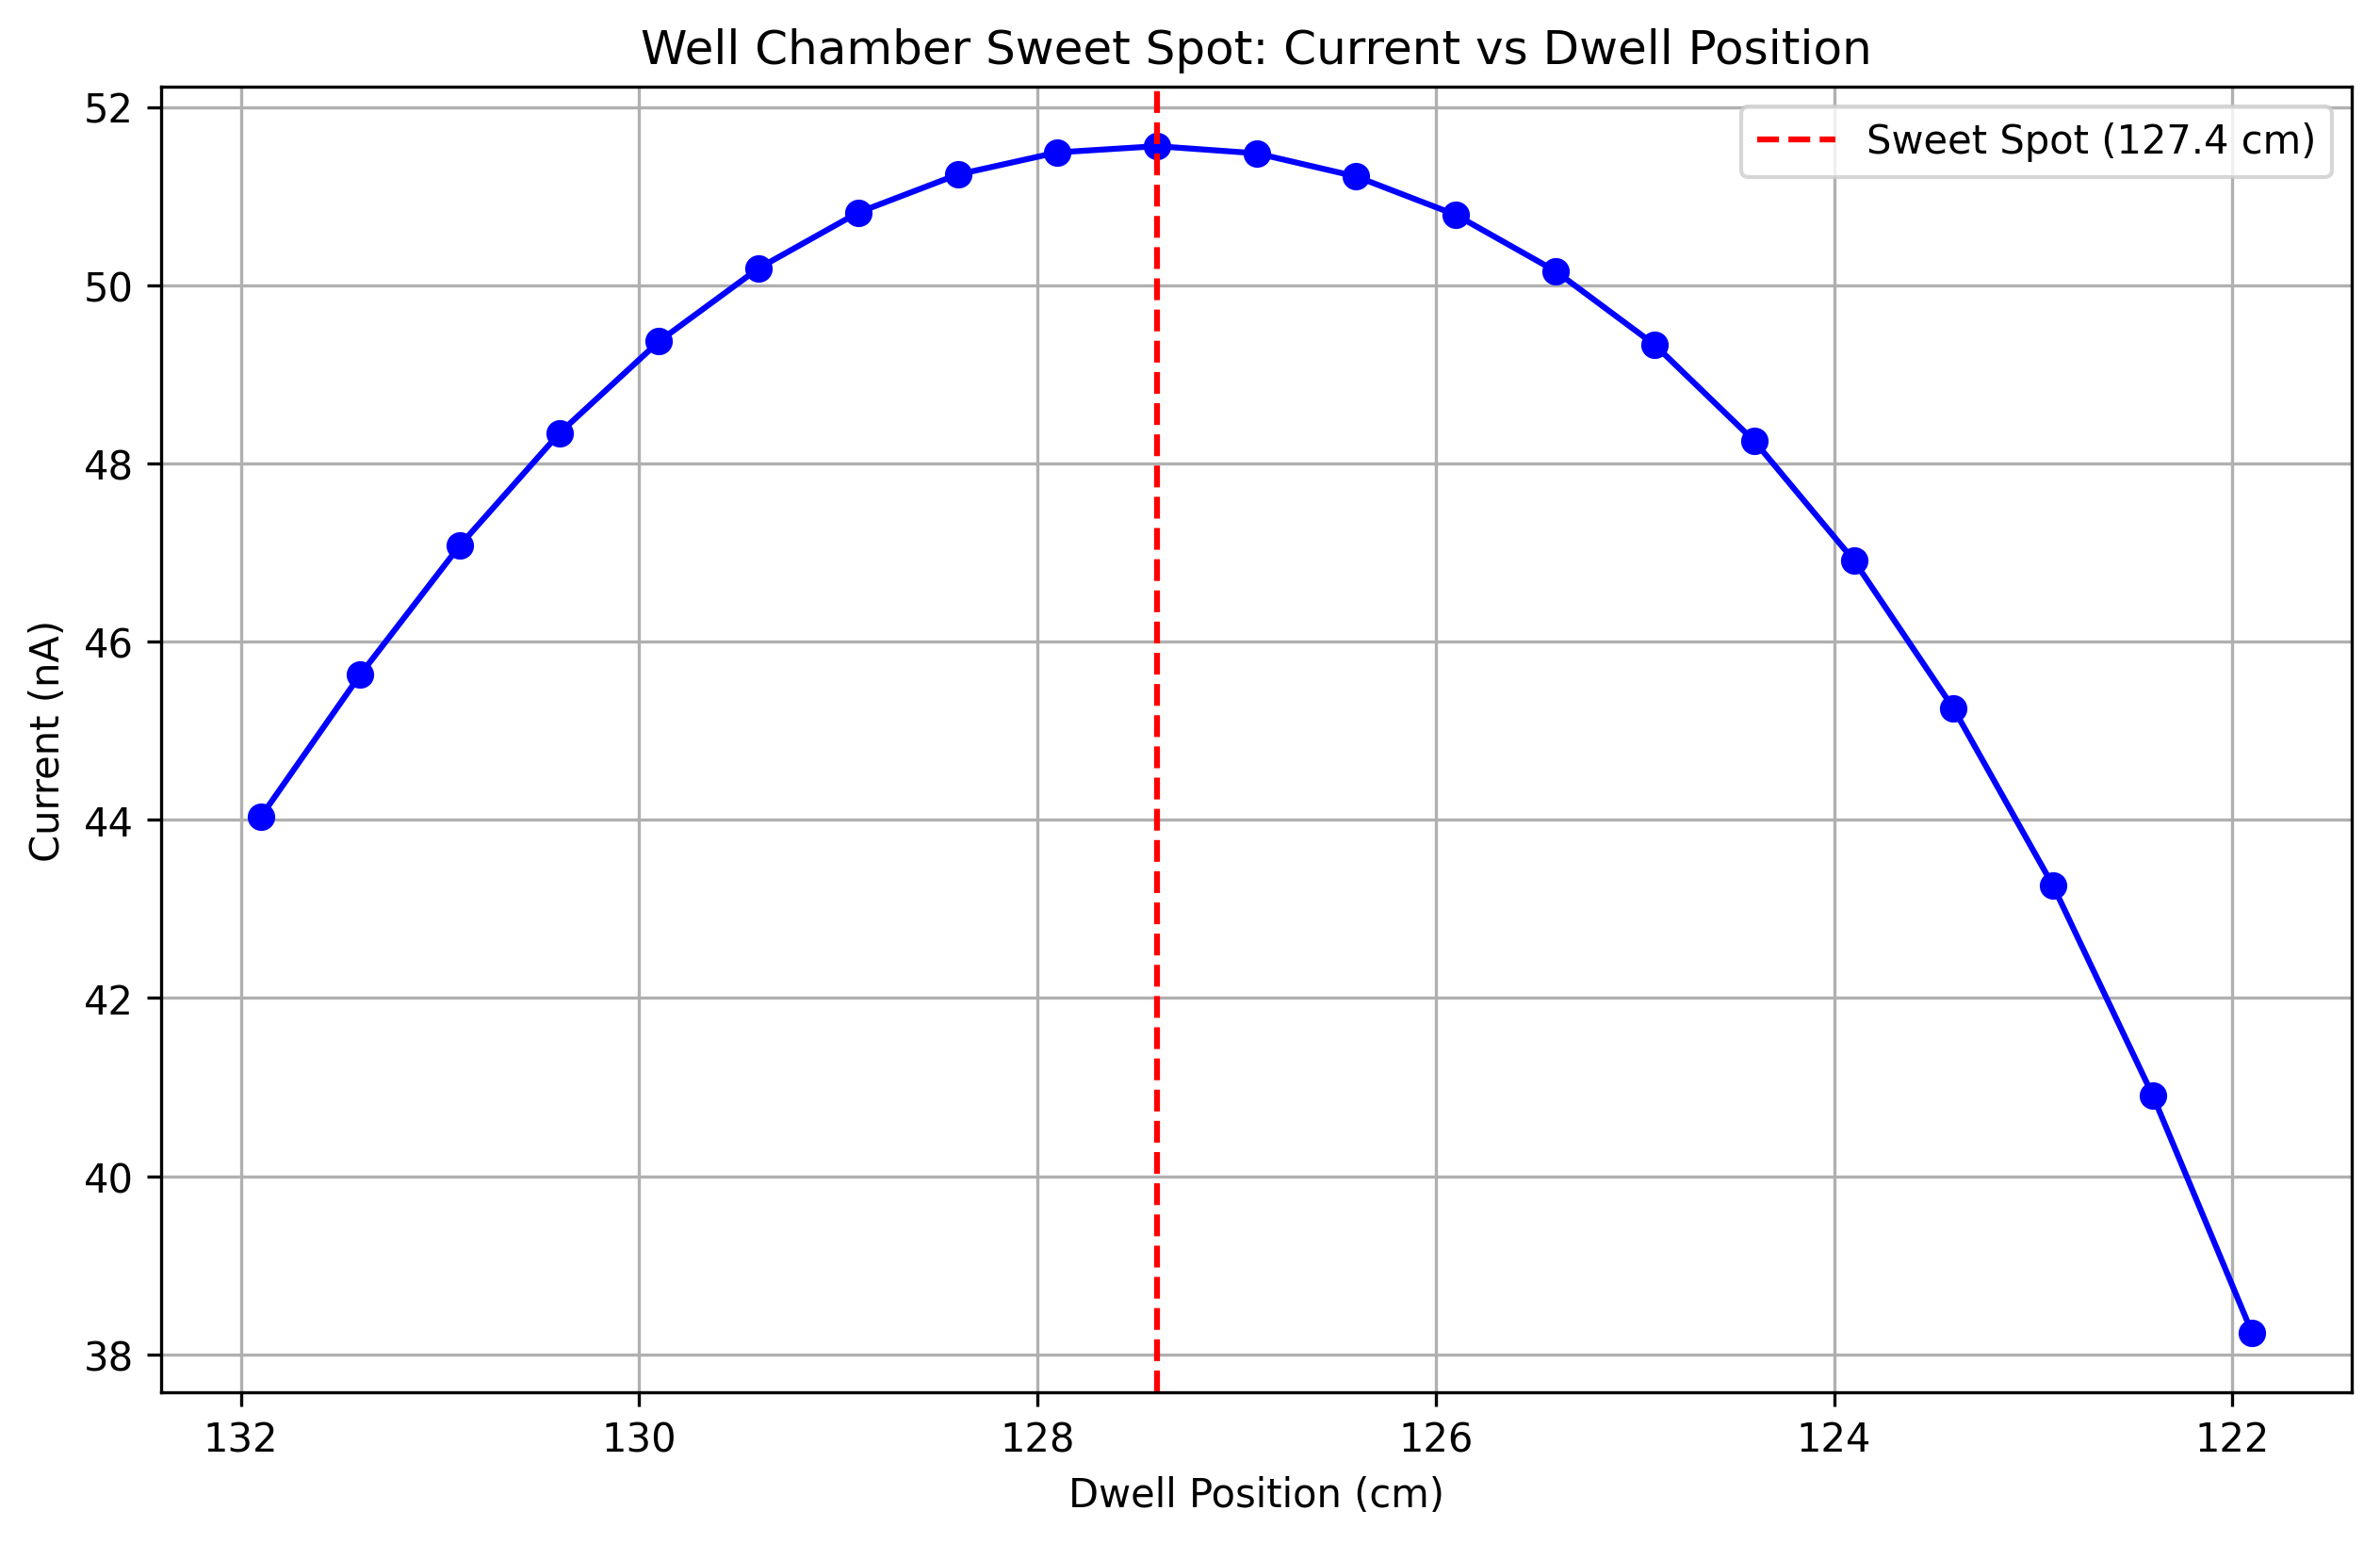
\includegraphics[width=0.8\textwidth]{Figures/sweet_spot_plot.png}
    \caption{Response curve defining the sweet spot.}
\end{figure}

Analysis of the response curve clearly indicates a maximum signal intensity at a dwell position of 127.4 cm, generating a peak current of 51.56 nA. This location, mapped to dwell channel number 10, was subsequently utilized for all primary strength measurements.

\subsection{Evaluation of Source Strength}
With the source localized at the predetermined sweet spot (127.4 cm, channel 10), three independent readings of 20 seconds duration were recorded to ensure statistical reliability.

\begin{table}[H]
    \centering
    \caption{Electrometer readings at the optimal sweet spot.}
    \begin{tabular}{|c|c|c|c|c|c|}
        \hline
        \textbf{Dwell Pos.} & \textbf{Polarity (V)} & \multicolumn{3}{c|}{\textbf{Current (nA)}} & \textbf{Avg. Current (nA)} \\
         & & \textbf{Trial 1} & \textbf{Trial 2} & \textbf{Trial 3} & \\
        \hline
        10 & -300 & 51.52 & 51.52 & 51.52 & 51.52 \\
        10 & +150 & 51.44 & 51.44 & 51.44 & 51.44 \\
        10 & +300 & 51.52 & 51.52 & 51.52 & 51.52 \\
        \hline
    \end{tabular}
\end{table}

\subsubsection{Derivation of Correction Factors}
To derive the true meter reading, several necessary correction factors must be computed based on operational parameters.

\textbf{1. Temperature and Pressure Correction ($K_{TP}$)}
Given local conditions of $T = 23.5^\circ$C and $P = 1010$ mb against reference states $T_0 = 20^\circ$C and $P_0 = 1013.2$ mb:
\begin{equation}
K_{TP} = \left( \frac{23.5 + 273.15}{20 + 273.15} \right) \cdot \left( \frac{1013.2}{1010} \right) = 1.015
\end{equation}

\textbf{2. Polarity Correction ($K_P$)}
Utilizing readings from opposing polarities ($\pm 300$V) referenced to the calibration polarity (+300V):
\begin{equation}
K_P = \frac{51.52 + 51.52}{2 \times 51.52} = 1.000
\end{equation}

\textbf{3. Ion Recombination Correction ($K_S$)}
Derived via the two-voltage technique (300V vs 150V):
\begin{equation}
K_S = \frac{4}{3} - \frac{51.52}{3 \times 51.44} = 1.0005
\end{equation}

\textbf{4. Electrometer Factor ($K_E$)}
Given that the chamber and electrometer were calibrated as a unified pair, $K_E = 1.000$.

The final corrected reading ($\dot{M}_{corr}$) is:
\begin{equation}
\dot{M}_{corr} = 51.52 \text{ nA} \times 1.015 \times 1.000 \times 1.0005 \times 1.000 = 52.32 \text{ nA}
\end{equation}

\subsubsection{RAKR and Source Activity Computation}
Using the provided calibration factor $N_K = 4.615 \times 10^5 \text{ Gy h}^{-1} \text{ A}^{-1}$:
\begin{equation}
\text{RAKR} = 52.32 \times 10^{-9} \text{ A} \times 4.615 \times 10^5 \text{ Gy h}^{-1} \text{ A}^{-1} = 24.1456 \text{ mGy h}^{-1}
\end{equation}

Converting this to apparent Activity ($A$) utilizing the specific air-kerma rate constant: $$\Gamma_\delta = 4.07114 \text{ mGy m}^2 \text{ h}^{-1} \text{ Ci}^{-1}$$
\begin{equation}
A = \frac{24.1456 \times (1)^2}{4.07114} = 5.931 \text{ Ci}
\end{equation}

\subsection{Timer Error Determination}
The intrinsic error associated with source transit and timer delay was evaluated using an interruption methodology over a 60-second exposure. The cumulative charge was compared between a continuous 60s run ($R_1$) and an equivalent run deliberately halted midway at 30s ($R_2$).

\begin{table}[H]
    \centering
    \caption{Charge accumulation for timer error test.}
    \begin{tabular}{|l|c|c|c|}
        \hline
        \textbf{Mode} & \textbf{Trial 1 ($\mu$C)} & \textbf{Trial 2 ($\mu$C)} & \textbf{Average ($\mu$C)} \\
        \hline
        Uninterrupted ($R_1$) & 3.103 & 3.103 & 3.103 \\
        Interrupted ($R_2$) & 3.146 & 3.146 & 3.146 \\
        \hline
    \end{tabular}
\end{table}

The resulting Timer Error is given by:
\begin{equation}
\text{Error} = \frac{(R_2 - R_1) \times t}{2 \times R_1 - R_2} = \frac{(3.146 - 3.103) \times 60}{2(3.103) - 3.146} = 0.8431 \text{ s}
\end{equation}

\subsection{Timer Linearity and End Error Assessment}
Timer proportionality was checked across varying set durations relative to a known constant current ($I = 0.05148 \text{ }\mu\text{A}$, established via a 300s dwell delivering $12.356 \text{ }\mu\text{C}$ over a measured 240s window).

\begin{table}[H]
    \centering
    \caption{Linearity check via variable dwell times.}
    \begin{tabular}{|c|c|c|}
        \hline
        \textbf{Set Time (s)} & \textbf{Average Charge ($\mu$C)} & \textbf{Measured Time (s) = Charge/Current} \\
        \hline
        60 & 3.103 & 60.27 \\
        120 & 6.190 & 120.24 \\
        180 & 9.277 & 180.20 \\
        240 & 12.365 & 240.19 \\
        300 & 15.456 & 300.23 \\
        \hline
    \end{tabular}
\end{table}

\begin{figure}[H]
    \centering
    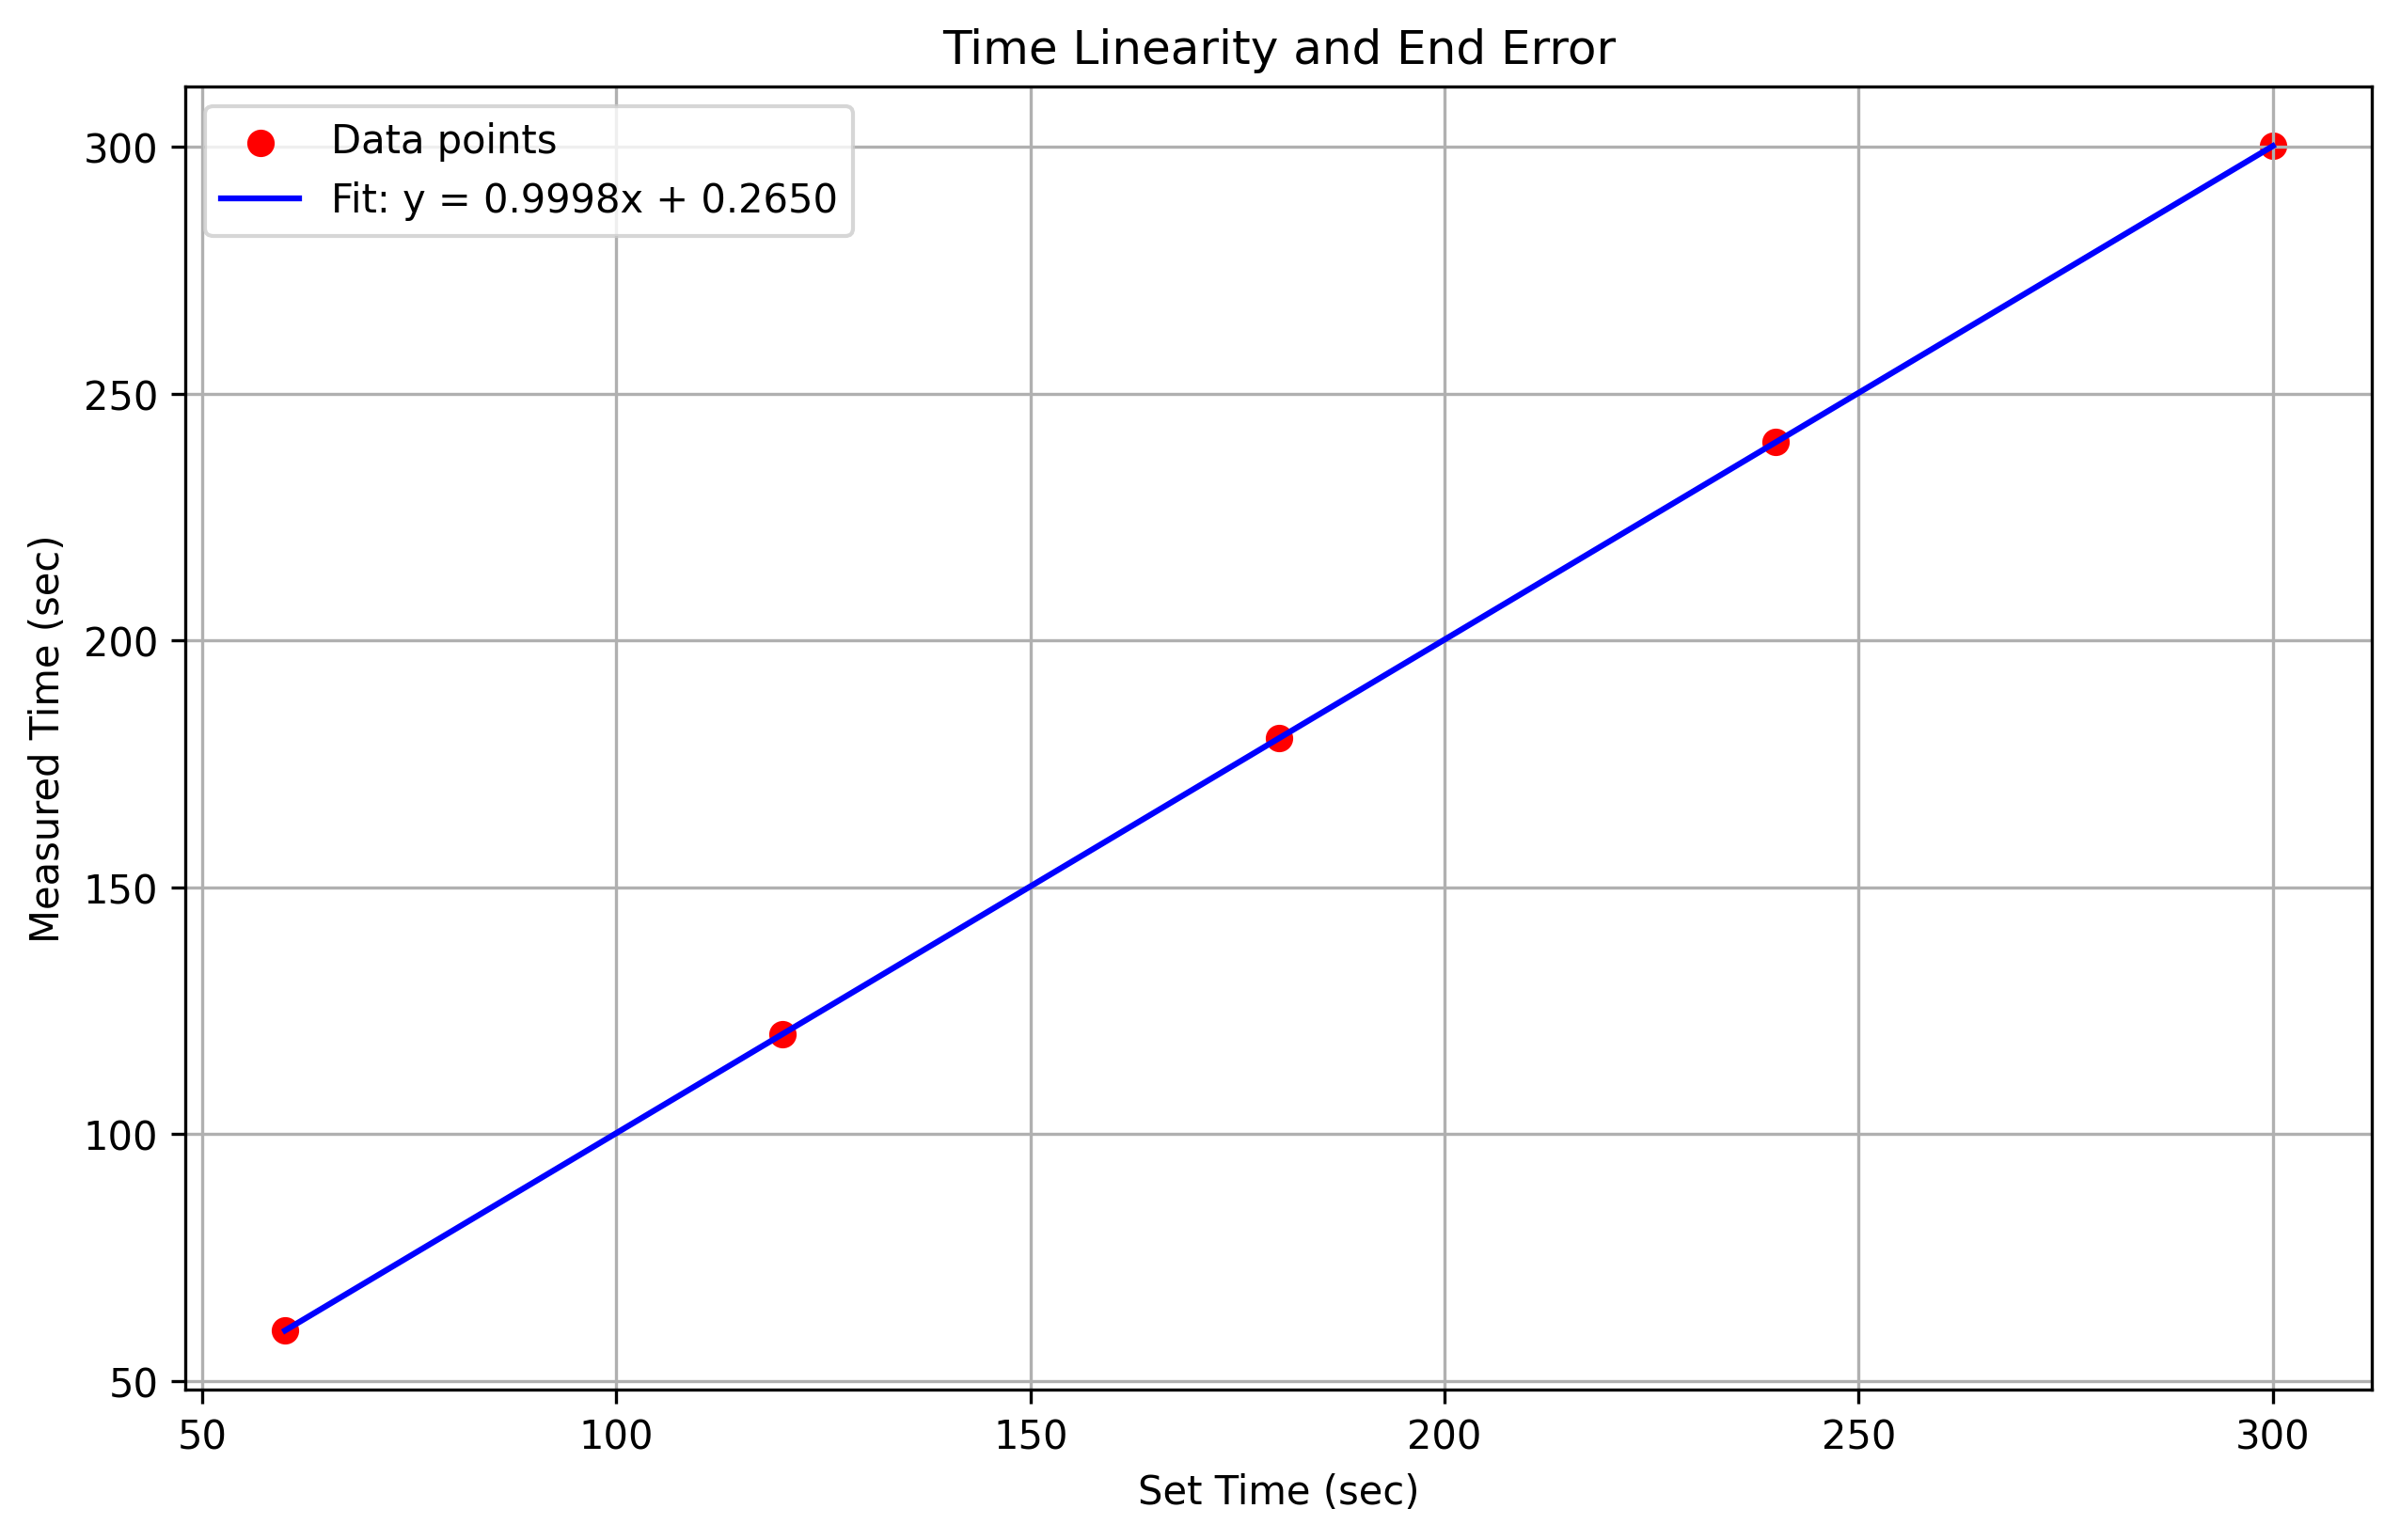
\includegraphics[width=0.8\textwidth]{Figures/time_linearity_plot.png}
    \caption{Timer linearity regression analysis.}
\end{figure}

Applying a linear fit to the measured data yields:
\begin{equation}
\text{Measured Time} = 0.9998 \cdot (\text{Set Time}) + 0.2650
\end{equation}
The derived metrics are therefore:
\begin{itemize}
    \item \textbf{End Error (Y-intercept):} 0.2650 s
    \item \textbf{Percentage Time Linearity Error:} $|1 - 0.9998| \times 100\% = 0.02\%$
\end{itemize}